% SABER AAAI-27 Korean submission skeleton.
% This file is intentionally separated from saber_aaai27_draft_kr.tex.
% Goal: keep the main submission self-contained and close to AAAI page limits.
% English page-limited submission skeleton.

\documentclass[letterpaper]{article}
\usepackage[submission]{aaai2027}
\usepackage[hyphens]{url}
\usepackage{graphicx}
\graphicspath{{./}{../}}
\urlstyle{rm}
\def\UrlFont{\rm}
\usepackage{natbib}
\usepackage{caption}
\frenchspacing

\usepackage{amsmath}
\usepackage{amssymb}
\usepackage{booktabs}

\ifdefined\pdfinfo
\pdfinfo{
/TemplateVersion (2027.1)
}
\fi

\setcounter{secnumdepth}{0}
\setcounter{dbltopnumber}{3}
\renewcommand{\dbltopfraction}{0.95}
\renewcommand{\textfraction}{0.05}

\newcommand{\ours}[1]{\textbf{#1 (Ours)}}
\newcommand{\oursnum}[1]{\(\boldsymbol{#1}\)}
\newcommand{\ourscell}[1]{\textbf{#1}}

\title{SABER: Support-Conditioned Adaptive Bellman Error Reweighting for Sparse HER Actor-Critic}
\author{Anonymous Submission}
\affiliations{}

\begin{document}
\maketitle

\begin{center}
\small\textbf{Content Areas:}\\
ML: Reinforcement, Imitation \& Inverse RL (primary);\\
ROB: Robot Learning, Control \& Foundation Models (secondary)
\end{center}
% Keep these labels synchronized with the OpenReview selections and add the paper ID once assigned.

\begin{abstract}
Existing HER improvements primarily decide which goals, transitions, or targets are used for learning; policy-query-conditioned post-relabeling critic supervision allocation remains implicit.
SABER exposes this complementary design axis by reweighting only critic Bellman residuals according to local support of the current policy action, while preserving relabeling, replay sampling, actor optimization, Bellman targets, critic architecture, and the one-update budget.
Under matched one-update budgets, SABER raises mean FetchPickAndPlace AUC across DDPG, TD3, and SAC; the TD3/SAC five-seed AUC intervals exclude zero, and a frozen ten-seed TD3 extension yields a paired AUC gain of $+0.0467\,[0.0085,0.0783]$.
In a matched TD3 query ablation, the current-policy query exceeds replay-action and sample-shuffled policy queries by $+0.075$ and $+0.096$ AUC, respectively. A stricter context-eligible count-matched control removes the positive-count confound and yields a $+0.052$ Main-minus-control AUC estimate on 4/5 seeds, although its interval includes zero. On DDPG and TD3, SABER also obtains AUC comparable to $4\times$ replay-ratio HER with one quarter of the gradient-update budget.
\end{abstract}

\section{Introduction}

Sparse-reward goal-conditioned RL is dominated by the question of how to obtain useful training signal when successes are rare. HER addresses this by relabeling failed trajectories with achieved goals~\citep{andrychowicz2017her}, turning failures into additional goal-conditioned Bellman targets. However, HER chooses \emph{which goals} to train on; it does not decide whether every relabeled Bellman residual is equally useful for fitting the critic near the action currently queried by the actor.

This distinction matters in off-policy actor-critic. The critic regresses Bellman targets at replay actions, while the actor improves by querying the critic at current policy actions. If the current policy action lies outside the local replay-action support for the same state-goal context, critic estimates in the actor-query region may be more fragile. We do not claim that this is a theorem or that support-positive targets are intrinsically lower-noise. Instead, we study local replay-action support as a policy-relevant proxy for allocating critic fitting pressure after HER.

SABER isolates post-HER critic supervision allocation as a complementary design axis. It reweights only the critic Bellman loss while preserving HER relabeling, replay sampling, actor optimization, backbone targets, critic architecture, and updates per step. This architecture-, replay-, and update-budget-preserving intervention supports cleaner effect attribution than changing several learning modules together. We study it under the standard one-update-per-step regime, with high replay-ratio HER and REDQ-HER as scaling references.

Our contributions are:
\begin{itemize}
    \item \textbf{Problem:} We identify post-HER critic supervision allocation as a distinct design axis from goal relabeling, replay prioritization, and Bellman-target construction.
    \item \textbf{Method:} We introduce an architecture-preserving, critic-only objective that allocates fitting pressure using local support of the current policy action.
    \item \textbf{Evidence:} We demonstrate cross-backbone repeatability, establish the value of sample-aligned current-policy querying over replay and shuffled alternatives, directly test membership-aligned assignment with per-update count matching, and show a favorable DDPG/TD3 update-budget trade-off plus a large-effect DrawerOpen rescue.
\end{itemize}

\begin{figure*}[t]
\centering
\setlength{\fboxsep}{5pt}
\small
\begin{tabular}{c@{\hspace{0.45em}$\rightarrow$\hspace{0.45em}}c@{\hspace{0.45em}$\rightarrow$\hspace{0.45em}}c@{\hspace{0.45em}$\rightarrow$\hspace{0.45em}}c}
\fbox{\parbox[c][1.82cm][c]{0.19\textwidth}{\centering\textbf{1. HER batch}\\[-1pt]\(o_i,a_i^r,g_i^{tr},r_i,o'_i,d_i\)\\relabeling unchanged}} &
\fbox{\parbox[c][1.82cm][c]{0.19\textwidth}{\centering\textbf{2. Local replay pool}\\[-1pt]\(c_i=C(o_i,g_i^{tr},h_i)\)\\\(\mathcal L_i\rightarrow\mathcal B_i\)}} &
\fbox{\parbox[c][1.82cm][c]{0.19\textwidth}{\centering\textbf{3. Policy-query path}\\[-1pt]\textbf{Query:} \(a_i^\pi\rightarrow b_i^\pi\)\\[-1pt]\(b_i^\pi\in\mathcal B_i\Rightarrow\psi_i\)\\[-1pt]\(w_i^{raw}\rightarrow\Omega_i\)}} &
\fbox{\parbox[c][1.82cm][c]{0.19\textwidth}{\centering\textbf{4. Replay-regression path}\\[-1pt]\textbf{Regress at:} \(a_i^r\)\\[-1pt]\(\Omega_i(Q_\phi(x_i,a_i^r)-y_i)^2\)\\actor loss unchanged}}
\end{tabular}
\vspace{0.35em}

\fbox{\parbox{0.94\textwidth}{\centering\small
\textbf{Changed:} sample-wise critic TD-loss allocation.\quad
\textbf{Unchanged:} HER goal generation, replay sampling, Bellman targets, actor objective, and critic architecture.}}
\caption{SABER intervenes after HER relabeling and before critic-loss aggregation. Stage 3 uses the current-policy action only to query local support; Stage 4 keeps Bellman regression at the replay action.}
\label{fig:saber-method-overview-submission}
\end{figure*}

\section{Related Work and Scope}

HER and later goal-conditioned methods improve sparse reward learning by changing how training goals, episodes, transitions, or targets are produced~\citep{andrychowicz2017her,ren2019hgg,fang2019cher,zhao2018ebp,luu2021hgr,yang2021mher}. HGR combines TD-error episode/goal sampling with importance correction; our FPP matched row implements this mechanism under the local DDPG+HER backbone, while Drawer rows keep only the sampler and are labeled accordingly. ARCHER rescales hindsight rewards, while USHER uses an importance ratio to correct HER Bellman bias~\citep{lanka2018archer,schramm2023usher}. ReF-ER suppresses gradients from far-policy replay samples and regularizes the policy toward replay behavior~\citep{novati2019refer}. SABER instead rejects no samples and does not constrain the actor; it keeps rewards, replay sampling, and one-step targets fixed while applying a local-support weight only to critic residuals.

PER prioritizes large TD-error samples~\citep{schaul2015per}. SABER does not rank by TD-error magnitude; its signal is local support of the current policy action. We nevertheless include PER-style and diagnostic comparisons because support-positive samples can be enriched among high-error samples. REDQ and sparse-goal REDQ-HER use high update-to-data ratios and Q ensembles~\citep{chen2021redq,hiraoka2023sparsegoalredq}; these are important compute/backbone-scaled references but are outside SABER's matched-backbone regime. The actor-critic backbones are DDPG, TD3, and SAC~\citep{lillicrap2015ddpg,fujimoto2018td3,haarnoja2018sac}. Experiments use Fetch and Meta-World manipulation tasks~\citep{plappert2018multigoal,yu2020metaworld}.

\section{Method}

For a replay transition \(i\), let \(x_i=(o_i,g_i^{tr})\) denote the unchanged actor-critic input, \(a_i^r\) the replay action, and \(a_i^\pi=\pi_\theta(o_i,g_i^{tr})\) the current policy action. Separately, \(c_i=C(o_i,g_i^{tr},h_i)\) denotes a support-only local context; the horizon feature \(h_i\) is not added to the actor or critic input. SABER builds a local pool \(\mathcal L_i\) of replay actions with the same discretized context and lets \(\mathcal B_i\) be its occupied action-bin set.

For FPP, \(C\) hashes an intended control phase, hand--object and object--goal distances, object height, gripper gap, and horizon. The other tasks use analogous task-specific stage and distance features; exact boundaries are provided in the supplement. Replay actions use \(K=5\) bins per action dimension. Main rows use \(N_{\mathrm{local}}=M_{\mathrm{avail}}=4\), \(M_B=16\), \(\lambda_S=1\), and deterministic-tail candidate lookup; FPP scans at most \(N_{\mathrm{scan}}=512\) replay entries per query. The support indicator is
\begin{align}
\psi_i={}&\mathbb{1}\{|\mathcal L_i|\ge N_{\mathrm{local}}\}
\mathbb{1}\{\min(|\mathcal L_i|,M_B)\ge M_{\mathrm{avail}}\}\notag\\
&\cdot \mathbb{1}\{b_i^\pi\in \mathcal B_i\}.
\end{align}
This predicate is a coarse action-bin membership proxy, not a density/diversity estimate or a direct target-noise estimator.

SABER maps \(\psi_i\) to a raw weight \(w_i^{raw}=1+\lambda_S\psi_i\), then batch-normalizes it:
\begin{equation}
\Omega_i=\frac{w_i^{raw}}{\frac{1}{|\mathcal B|}\sum_{j\in\mathcal B}w_j^{raw}}.
\end{equation}
For a one-step HER Bellman target \(y_i\) and critic \(Q_\phi\), the critic objective is
\begin{equation}
\mathcal L_Q(\phi)=\frac{1}{|\mathcal B|}\sum_{i\in\mathcal B}\Omega_i\left(Q_\phi(x_i,a_i^r)-y_i\right)^2.
\end{equation}
For TD3 and SAC, the same \(\Omega_i\) is applied to each critic's Bellman residual. Actor updates and target networks remain exactly those of the underlying backbone.

\section{Experimental Setup}

\paragraph{Why future-goal HER is the controlled base.}
We do not assume that HER is globally strongest across heterogeneous protocols. We select future-goal HER because it is canonical, composes unchanged with all three backbones, and leaves replay, targets, architecture, and UTD available for controlled intervention. Future sampling with \(k=4\) or 8 was strongest among the original study's tested strategies~\citep{andrychowicz2017her}; our 0.8 relabeling probability matches the expected \(4{:}1\) mixture of \(k=4\). Under matched FPP DDPG, HER reaches AUC \(0.539\pm0.125\) and Hit90 in 5/5 seeds versus matched HGR's \(0.338\pm0.149\) and 2/5 (Table~\ref{tab:fpp-main-submission}). Higher high-RR/REDQ-HER rows change UTD or architecture and remain scaling references (Table~\ref{tab:scaling-submission}).

We retain benchmark/wrapper horizons and one common budget within each task. FPP is the canonical sparse Fetch and primary cross-backbone test; DrawerOpen tests cross-suite, contact-rich rescue; DrawerClose reverses the motion and probes late stability rather than supplying a second primary positive result. The 1M/2M budgets do not equalize episode count, compute, or difficulty across suites.

All matched rows use two-layer 256-unit MLPs, a 300k replay buffer, 5k-step warmup, 10k random-start steps, and Adam with actor/critic learning rates \(3\times10^{-4}\), \(\gamma=0.98\), and target-update coefficient \(\tau=0.005\). Successful relabels remain nonterminal in Bellman targets, and time-limit transitions bootstrap.

\begin{table}[t]
\centering
\scriptsize
\setlength{\tabcolsep}{3pt}
\caption{Task settings and evidential roles. Horizon/budget are fixed within task.}
\label{tab:design-rationale-submission}
\begin{tabular}{@{}lccp{0.25\columnwidth}@{}}
\toprule
Task & Horizon & Budget & Role \\
\midrule
FPP & 50 & 1M & cross-backbone main \\
DrawerOpen & 200 & 2M & cross-suite rescue \\
DrawerClose & 200 & 2M & stability boundary \\
\bottomrule
\end{tabular}
\end{table}

Main Fetch rows use seeds \(1,\ldots,5\), HER ratio 0.8, batch size 256, and 20 evaluation episodes. FPP SAC AUC and Hit90 use the exact shared grid \(\{50\mathrm{k},\ldots,1\mathrm{M}\}\) with no interpolation or filling; this removes the legacy 25k versus newer 10k evaluation-frequency mismatch. Steps/sec and runtime are observed, not hardware-normalized claims.

The central comparison is matched-backbone one-update-per-step HER versus HER+SABER. Controls include matched HGR, PER/random variants, high replay-ratio HER, REDQ-HER, and diagnostics. The TD3 query ablation changes only the query action; the strict assignment control matches context eligibility, same-trajectory counterfactual Main count, and weight histograms per update. Drawer HGR-style rows remain sampler-only stress ablations; HGG/MHER/CHER are not directly compared.

\section{Results}

\subsection{Cross-Backbone Repeatability}

\textbf{SABER produces a repeatable cross-backbone improvement under matched one-update budgets.}

\begin{figure*}[t]
\centering
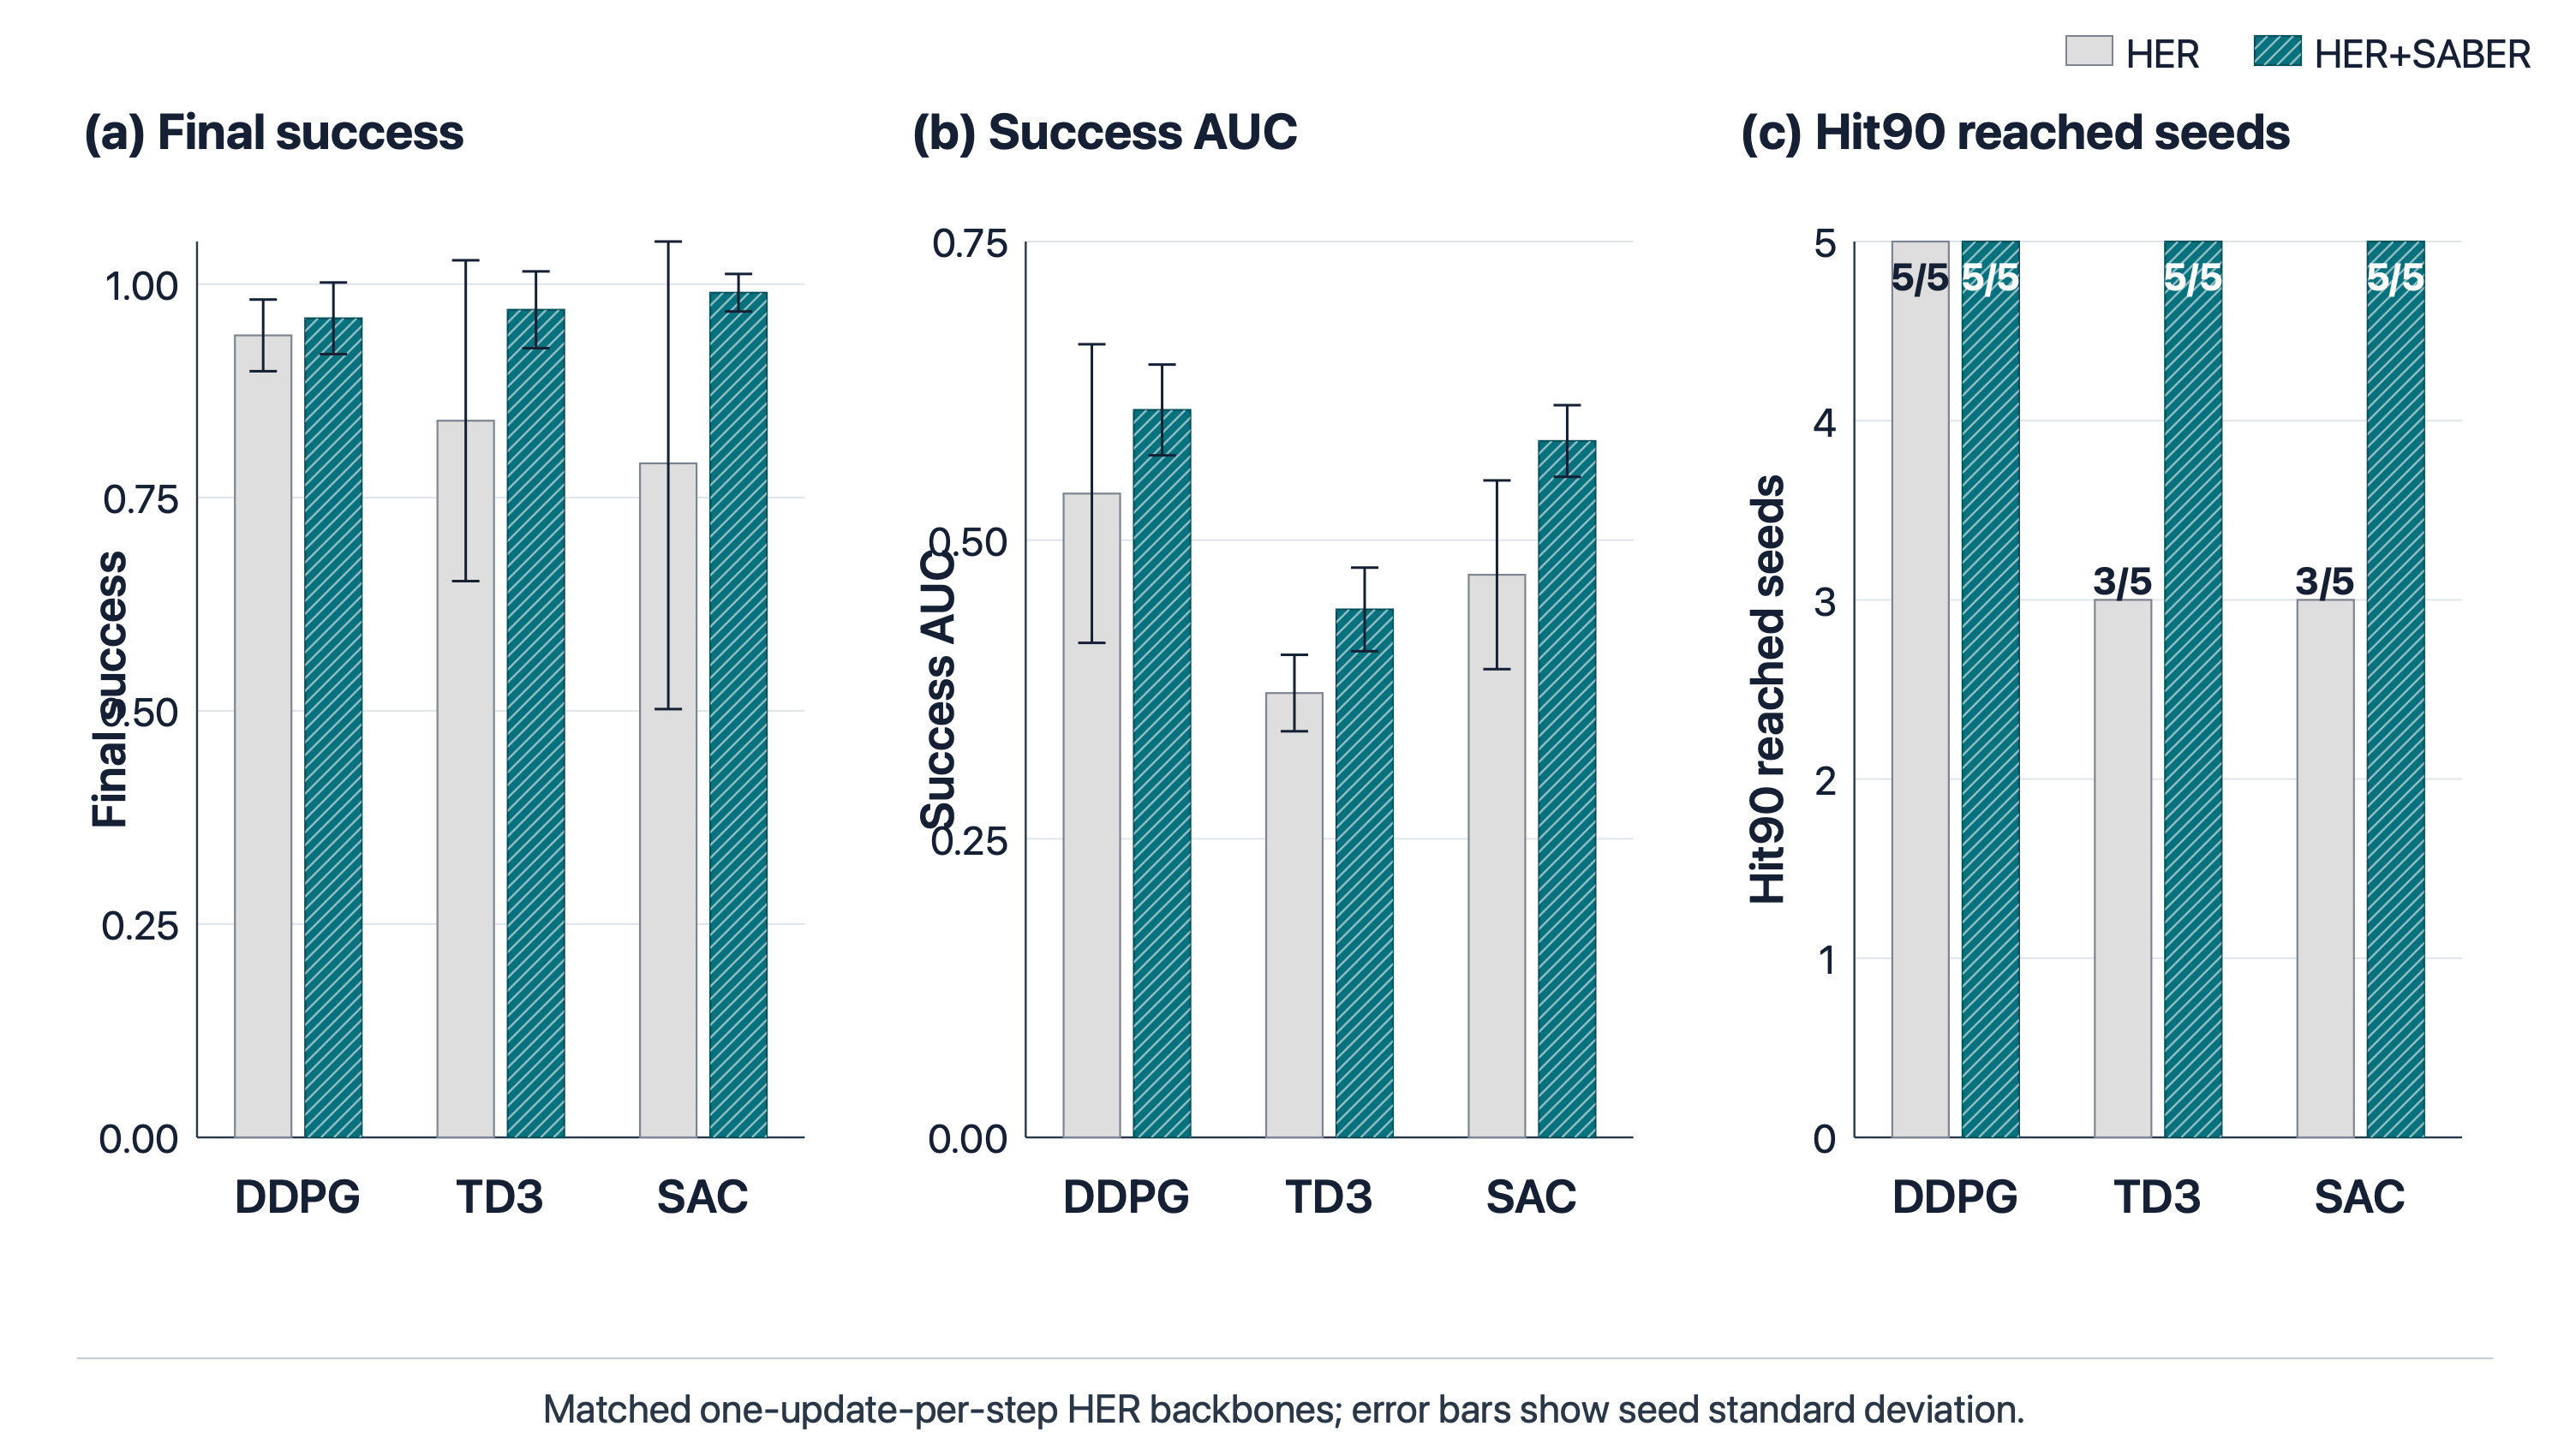
\includegraphics[width=0.98\textwidth]{output/figures/fpp_saber_main_evidence.png}
\caption{FetchPickAndPlace evidence across matched one-update-per-step HER backbones. Bars and error bars show the seed mean and standard deviation. Exact paired 95\% SABER--HER intervals are reported in Table~\ref{tab:fpp-main-submission}; the AUC interval includes zero for DDPG and excludes zero for TD3/SAC.}
\label{fig:fpp-main-evidence-submission}
\end{figure*}

\begin{table*}[t]
\centering
\small
\caption{Matched-backbone comparison: FPP main results and matched HGR reference at 1M steps. SAC AUC and Hit90 use the exact shared 50k--1M grid. SABER improves means across all backbones; paired AUC CIs are clearer for TD3/SAC than DDPG.}
\label{tab:fpp-main-submission}
\begin{tabular}{llcccc}
\toprule
Backbone & Method & Final & AUC & Hit90 & Steps/sec \\
\midrule
DDPG & HER & \(0.940 \pm 0.042\) & \(0.539 \pm 0.125\) & 600k (5/5) & \(65.03\) \\
\ourscell{DDPG} & \ours{HER+SABER} & \oursnum{0.960 \pm 0.042} & \oursnum{0.609 \pm 0.038} & \ourscell{540k (5/5)} & \oursnum{41.72} \\
DDPG & HGR (matched) & \(0.540 \pm 0.365\) & \(0.338 \pm 0.149\) & 930k (2/5) & \(16.93\) \\
TD3 & HER & \(0.840 \pm 0.188\) & \(0.372 \pm 0.032\) & 980k (3/5) & \(65.33\) \\
\ourscell{TD3} & \ours{HER+SABER} & \oursnum{0.970 \pm 0.045} & \oursnum{0.442 \pm 0.035} & \ourscell{840k (5/5)} & \oursnum{41.25} \\
SAC & HER & \(0.790 \pm 0.288\) & \(0.471 \pm 0.079\) & 800k (3/5) & \(38.93\) \\
\ourscell{SAC} & \ours{HER+SABER} & \oursnum{0.990 \pm 0.022} & \oursnum{0.583 \pm 0.030} & \ourscell{750k (5/5)} & \oursnum{29.10} \\
\midrule
DDPG & \(\Delta\) SABER--HER & \(+0.020[-0.040,0.070]\) & \(+0.070[-0.016,0.193]\) & -- & -- \\
TD3 & \(\Delta\) SABER--HER & \(+0.130[-0.030,0.310]\) & \(+0.071[0.032,0.095]\) & -- & -- \\
SAC & \(\Delta\) SABER--HER & \(+0.200[-0.020,0.430]\) & \(+0.112[0.064,0.161]\) & -- & -- \\
\bottomrule
\end{tabular}
\end{table*}

SABER raises mean FPP AUC from 0.539 to 0.609 on DDPG, 0.372 to 0.442 on TD3, and 0.471 to 0.583 on SAC. The paired AUC intervals exclude zero for TD3 and SAC, and all three backbones improve in mean final success and Hit90 coverage. This demonstrates cross-backbone compatibility rather than a single-backbone anomaly.

\paragraph{Ten-seed TD3 confirmation.}
A frozen paired extension on seeds 6--10 gives ten matched TD3 pairs on the exact 10k--1M grid. HER versus SABER reaches AUC $0.383\pm0.041$ versus $0.429\pm0.058$, with paired delta $+0.0467[0.0085,0.0783]$; 8/10 seed deltas are positive and every leave-one-out mean remains positive. The extension corroborates the five-seed result while preserving its finite-seed boundary: DDPG supplies mean-improvement rather than interval-closed evidence, and neither result implies improvement on every seed.

\subsection{Policy-Aligned Querying Is Substantive}

\textbf{The support query is not interchangeable with replay-action querying or sample-misaligned policy querying.}

\begin{table*}[t]
\centering
\small
\caption{FPP TD3 mechanism controls at 1M steps, seeds 1--5. Paired 95\% CIs compare Main with each row. The strict control samples \(k=|M|\) positions from \(E\) on each control update; context-count only is count-unmatched.}
\label{tab:query-ablation-submission}
\begin{tabular}{lcccc}
\toprule
Query / control & Final & AUC & Hit90 & Main $-$ row AUC [CI] \\
\midrule
HER & \(0.840\pm0.188\) & \(0.372\pm0.032\) & 980k (3/5) & \(+0.071[0.032,0.095]\) \\
\ours{Main SABER} & \oursnum{0.970\pm0.045} & \oursnum{0.442\pm0.035} & \ourscell{840k (5/5)} & \ourscell{--} \\
Replay action & \(0.660\pm0.219\) & \(0.368\pm0.042\) & 920k (1/5) & \(+0.075[0.059,0.092]\) \\
Shuffled policy & \(0.550\pm0.226\) & \(0.347\pm0.051\) & 890k (1/5) & \(+0.096[0.063,0.128]\) \\
\shortstack[l]{Context-eligible\\count-matched} & \(0.910\pm0.096\) & \(0.391\pm0.070\) & 955k (4/5) & \(+0.052[-0.016,0.099]\) \\
Context-count only & \(0.800\pm0.242\) & \(0.396\pm0.090\) & 850k (3/5) & \(+0.047[-0.041,0.122]\) \\
\bottomrule
\end{tabular}
\end{table*}

The main current-policy query exceeds replay-query and shuffled-policy on every paired seed. Replay-query has a higher support-positive rate than Main (0.426 versus 0.219) yet lower AUC, while shuffling preserves the policy-action marginal distribution but removes sample alignment. Thus query identity and sample alignment matter beyond merely producing more support-positive weights.

\textbf{Count-matched assignment.} Each control update recomputes \(E,M,k\) and samples \(Z\subseteq E\), \(|Z|=k\), without using membership locations; instrumented summaries record no count or weight-distribution violations. Main versus control AUC is \(0.4424\pm0.0350\) versus \(0.3908\pm0.0700\), with paired difference \(+0.0516[-0.0165,0.0992]\), 4/5 positive seeds, and exact \(p=0.25\). This removes the count confound and directionally favors membership alignment, but does not confirm its independent contribution.

\subsection{A Favorable Gradient-Update Trade-Off}

\textbf{On DDPG and TD3, SABER reaches AUC comparable to $4\times$ replay-ratio HER with one quarter of the gradient-update budget.}

\begin{table*}[t]
\centering
\small
\caption{Scaling references: FPP SAC/REDQ metrics use the exact shared 50k--1M grid. High-RR and REDQ rows expose update/backbone budget tradeoffs.}
\label{tab:scaling-submission}
\begin{tabular}{llccccc}
\toprule
Backbone & Method & Updates/step & Final & AUC & Hit90 & Runtime h \\
\midrule
\ourscell{DDPG} & \ours{HER+SABER} & \ourscell{1} & \oursnum{0.960 \pm 0.042} & \oursnum{0.609 \pm 0.038} & \ourscell{540k (5/5)} & \ourscell{6.66} \\
DDPG & HER high-RR \(4\times\) & 4 & \(0.990 \pm 0.022\) & \(0.618 \pm 0.071\) & 480k (5/5) & 16.11 \\
DDPG & HER high-RR \(8\times\) & 8 & \(0.720 \pm 0.407\) & \(0.443 \pm 0.269\) & 620k (3/5) & 31.85 \\
\ourscell{TD3} & \ours{HER+SABER} & \ourscell{1} & \oursnum{0.970 \pm 0.045} & \oursnum{0.442 \pm 0.035} & \ourscell{840k (5/5)} & \ourscell{6.74} \\
TD3 & HER high-RR \(4\times\) & 4 & \(0.610 \pm 0.243\) & \(0.449 \pm 0.079\) & 630k (1/5) & 8.76 \\
\ourscell{SAC} & \ours{HER+SABER} & \ourscell{1} & \oursnum{0.990 \pm 0.022} & \oursnum{0.583 \pm 0.030} & \ourscell{750k (5/5)} & \ourscell{9.55} \\
SAC & HER high-RR \(4\times\) & 4 & \(0.960 \pm 0.042\) & \(0.768 \pm 0.097\) & 450k (5/5) & 47.02 \\
REDQ-SAC & REDQ-HER TQB & 4 & \(1.000 \pm 0.000\) & \(0.867 \pm 0.052\) & 300k (5/5) & 89.52 \\
\bottomrule
\end{tabular}
\end{table*}

For TD3, comparable AUC is accompanied by substantially higher final success (0.970 versus 0.610) and Hit90 coverage (5/5 versus 1/5). SABER therefore offers a complementary one-update allocation strategy rather than relying on brute-force replay scaling. \textbf{Boundary:} this is a gradient-update trade-off, not a wall-clock-efficiency claim; SAC high-RR and REDQ-HER TQB attain higher AUC with larger update or architecture budgets.

\subsection{Large-Effect Rescue on DrawerOpen}

\textbf{SABER rescues a failure-prone HER regime on DrawerOpen.} It raises final success from 0.390 to 1.000, AUC from 0.207 to 0.754, and Hit90 coverage from 2/5 to 5/5 seeds. This shows that critic-side allocation can have a large practical effect when matched HER suffers from seed-level failures.

\begin{table*}[t]
\centering
\small
\caption{DrawerOpen stress case at 2M steps. DDPG rows use the local matched regime; REDQ-HER TQB is an N=10, M=2, UTD-4 architecture/compute-scaled reference. Hit90 reports median first hit and reached seeds.}
\label{tab:drawer-hgr-submission}
\begin{tabular}{lccc}
\toprule
Method & Final & AUC & Hit90 \\
\midrule
HER & \(0.390\pm0.534\) & \(0.207\pm0.287\) & 960k (2/5) \\
HGR-style sampler-only & \(0.400\pm0.548\) & \(0.311\pm0.425\) & 450k (2/5) \\
\ours{HER+SABER} & \oursnum{1.000\pm0.000} & \oursnum{0.754\pm0.044} & \ourscell{500k (5/5)} \\
Random-support & \(1.000\pm0.000\) & \(0.706\pm0.122\) & 510k (5/5) \\
PER-style & \(0.800\pm0.447\) & \(0.715\pm0.090\) & 610k (5/5) \\
REDQ-HER TQB (scaled) & \(1.000\pm0.000\) & \(0.672\pm0.314\) & 370k (5/5) \\
\bottomrule
\end{tabular}
\end{table*}

Random-support and PER-style controls are also strong, so DrawerOpen establishes intervention-family significance rather than unique structured-support causality. The HGR-style sampler-only row reaches Hit90 in 2/5 seeds; SABER minus HGR-style is \(+0.443[0.106,0.780]\) in AUC, but the row is not full HGR. Scaled REDQ-HER TQB reaches Hit90 earlier (370k versus 500k median), whereas SABER has higher mean AUC and lower variance, \(0.754\pm0.044\) versus \(0.672\pm0.314\); neither method dominates every seed or metric.

An independent SABER-only extension reaches Hit90 in 4/5 additional seeds; descriptively pooled over seeds 1--10, SABER reaches 9/10 with final success \(0.895\pm0.315\) and AUC \(0.652\pm0.246\). Because no matched methods were extended, the original five-seed paired comparisons remain primary. A separate diagnostic rerun reproduces the original five-seed aggregate AUC (0.755 versus 0.754). Across nine successful diagnostic seeds, support-positive samples show 1.17\(\times\) pre-update TD error and 2.1\(\times\) same-minibatch residual reduction; failed seed 7 first loses contact exploration and later exhibits support saturation. These in-sample diagnostics characterize allocation and failure behavior rather than causal generalization.

\begin{table*}[t]
\centering
\small
\caption{Control closure: what the reported controls establish and what remains unresolved.}
\label{tab:closure-submission}
\begin{tabular}{p{0.29\textwidth}p{0.31\textwidth}p{0.31\textwidth}}
\toprule
Evidence & Established & Remaining interpretation \\
\midrule
DDPG controls: Random-fixed AUC 0.540 is close to HER 0.539; Random-support AUC 0.604 is close to SABER 0.609. &
Fixed-count random weighting alone does not explain the gain. &
FPP DDPG does not isolate exact sample-level alignment; count-preserving randomization can regularize. \\
\addlinespace
TD3/SAC random controls stay near or below SABER in AUC. &
Random reweighting does not explain all gains across backbones. &
TD3/SAC provide the cleanest random-control separation. \\
\addlinespace
High-RR/REDQ rows match or exceed SABER under larger budgets. &
SABER offers a distinct one-update allocation strategy. &
It does not dominate update or architecture scaling. \\
\addlinespace
FPP HGR (matched) uses pair priorities and episode/pair IS correction but reaches AUC 0.338 and Hit90 in 2/5; SABER reaches 0.609 and 5/5. &
Matched goal prioritization does not explain SABER's gain in this regime. &
This is not an exact original-paper reproduction or a general HGR ranking. \\
\addlinespace
Diagnostics show weak TD-error correlation, top-error enrichment, and larger immediate correction in TD3/SAC. &
SABER is not PER-style largest-error selection. &
The evidence supports error allocation, not lower target variance. \\
\addlinespace
Main query AUC 0.442 exceeds replay 0.368 and shuffled 0.347 on all five paired seeds; the context-eligible count-matched control reaches 0.391. &
Current-policy identity and sample alignment are substantive, and the strict control removes the positive-count/context-eligibility confound. &
Main--control is \(+0.052[-0.016,0.099]\) on 4/5 seeds; membership-specific benefit is directional but not interval-closed. \\
\bottomrule
\end{tabular}
\end{table*}

\FloatBarrier
\raggedbottom
\subsection{Mechanism Characterization and Boundaries}

\paragraph{Allocation diagnostics.}
Instrumented DDPG, TD3, and SAC runs log 500 full diagnostic batches and 64k sample rows per backbone. Support-positive rates are 0.367, 0.219, and 0.197, while Pearson correlations with \(|\delta|\) are only 0.116, 0.128, and 0.143. Their top-10\% TD-error overlaps are 0.516, 0.360, and 0.342: enriched over each support base rate but far from TD-error equivalence. TD3/SAC support-positive samples also receive larger immediate residual correction after weight normalization. Target variance is higher, not lower, in all three diagnostics, supporting an allocation signal rather than a lower-noise interpretation.

Together, the controls establish a distinct policy-aligned allocation signal on TD3/SAC and characterize where generic reweighting, goal prioritization, or scaling remain competitive. They define the operating regime of the contribution rather than displacing its core matched-budget findings.

\section{Discussion}

\subsection{What SABER Establishes}

SABER establishes post-HER critic supervision allocation as a distinct design axis. Holding relabeling, replay, actor optimization, Bellman targets, critic architecture, and update rate fixed provides cleaner effect attribution and a common interface across DDPG, TD3, and SAC. The evidence then localizes the signal: aligned current-policy querying exceeds replay and shuffled-policy queries, cross-backbone and ten-seed results show repeatability, DDPG/TD3 expose a favorable gradient-update trade-off, and DrawerOpen demonstrates that critic-side allocation can rescue a failure-prone HER regime.

\subsection{Scope and Limitations}

The evidence is scoped in five ways. First, the support predicate is task-specific and uses coarse membership; FetchSlide DDPG decreases from HER final/AUC \(0.630/0.324\) to SABER \(0.590/0.301\), and DrawerClose remains high variance. Second, query and membership assignment are tested only on FPP TD3. The strict context-eligible count-matched control removes the earlier count confound and favors Main in mean AUC, but its five-seed interval includes zero; a weakly active D8 gate also does not establish a diversity benefit. Third, diagnostics are in-sample allocation measurements, not lower-noise or causal-generalization proofs. Fourth, the current lookup is costly: in a hardware-specific seed-1 profile, TD3 throughput falls from 124.0 to 41.4 steps/s and support/weighting occupies 62.3\% of SABER's loop. Fifth, matched FPP HGR is not an exact original-paper reproduction, HGG/MHER/CHER remain untested, and most controls use five seeds.

\paragraph{Statistical scope.}
Paired deltas use 10,000 seed bootstrap resamples. Exact sign-flip tests for FPP DDPG/TD3/SAC AUC give $p=0.375/0.125/0.0625$, with positive deltas on 3/5, 4/5, and 5/5 seeds; all leave-one-out means remain positive. With five nonzero pairs, 0.0625 is the minimum attainable two-sided value. The ten-seed TD3 extension contains two negative deltas and exact $p=0.0527$, while the DrawerOpen extension is SABER-only and unmatched. These checks establish repeatability and outlier stability, not improvement on every seed.

\section{Conclusion}
SABER establishes post-HER critic supervision allocation as a design axis distinct from relabeling, replay, actor optimization, Bellman targets, architecture, and update rate. It yields a repeatable cross-backbone FPP signal, corroborated by the paired TD3 ten-seed extension, and aligned current-policy querying outperforms replay/shuffled alternatives. Count matching removes the earlier confound but does not interval-close the incremental membership effect. SABER also offers a DDPG/TD3 gradient-update trade-off and rescues a failure-prone DrawerOpen regime. Generic support representations remain future work.

\section{Reproducibility and Anonymity}

An anonymized archive provides sanitized configs, exact-grid curves, package-local analyzers/tests, and SHA256 manifests for the matched HGR, TD3 ten-seed, query/count-matched, DrawerOpen, scaling, and runtime evidence. Package commands regenerate compact tables; independent checks cover exact inference, leave-one-out, and table consistency. Public URLs, user namespaces, and raw commit identities are excluded.

\makeatletter
\@ifundefined{isChecklistMainFile}{\bibliographystyle{aaai2027}}{}
\makeatother
\bibliography{saber_refs}

\end{document}
